\subsection{Strategy}

O padrão Strategy define grupos de algoritmos encapsulados e
 intercambiáveis para um determinado contexto. Esses 
 algoritmos podem ser definidos ou trocados em tempo de 
 execução, permitindo que os clientes que os utilizem possam
  alternar entre as implementações definidas livremente.

O Strategy soluciona o problema de classes relacionadas 
diferirem apenas em algum comportamento, permitindo que 
esse comportamento possa ser isolado e o resto da implementação 
das classes reaproveitado. Ele também evita a utilização de 
muitas operações condicionais. Ao invés de verificar qual 
deve ser o comportamento toda vez que ele precisar ser 
executado, o comportamento é pré-definido pelo contexto.

\begin{figure}[htb]
	\caption{\label{fig_grafico}Estrutura do Strategy}
	\begin{center}
	    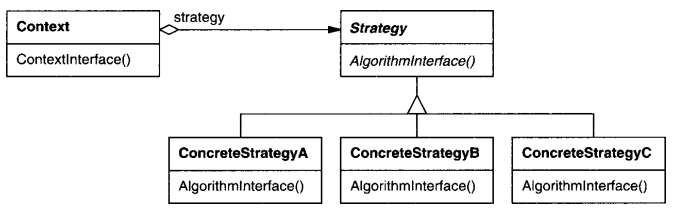
\includegraphics[scale=0.5]{5_padroes-contexto-funcional/5.3_comportamentais/5.3.09_strategy/diagram.png}
	\end{center}
\end{figure}

Exemplo Orientado a Objetos:

\begin{lstlisting}[caption={Strategy Orientação a Objetos},label=oostrategy]
    
    trait Strategy {
        def execute(a : Int, b : Int) : Int
    }

    class ConcreteStrategyAdd() extends Strategy {
        def execute(a : Int, b : Int) : Int = {
            a + b
        }
    }

    class ConcreteStrategySubtract() extends Strategy {
        def execute(a : Int, b : Int) : Int = {
            a - b
        }
    }

    class ConcreteStrategyMultiply() extends Strategy {
        def execute(a : Int, b : Int) : Int = {
            a * b
        }
    }

    class Context() {
        
        private var strategy : Strategy

        def setStrategy(strategy : Strategy) =
            this.strategy = strategy

        def executeStrategy(a : Int, b : Int) : Int =
            this.strategy.execute(a, b)

    }

\end{lstlisting}

Contexto Funcional:

No contexto funcional, o encapsulamento de algoritmos 
ou de comportamentos diferentes pode ser alcançado através 
de funções de alta ordem (high-order functions). Nesse caso,
 não é necessário definir interfaces ou objetos para encapsular 
 esses comportamentos, eles podem ser recebidos através da 
 passagem de parâmetro como funções:


\begin{lstlisting}[caption={Strategy Funcional},label=fpstrategy]
    
    def executeAdd(a : Int, b: Int) : Int = {
        a + b
    }

    def executeSubtract(a : Int, b: Int) : Int = {
        a - b
    }

    def executeMultiply(a : Int, b: Int) : Int = {
        a * b
    }

    def executeStrategy(execute : (a : Int, b : Int) => Int) : Int =
        execute(a, b)

\end{lstlisting}

Porém, existe uma desvantagem. A função [executeStrategy] 
acima aceita qualquer função que receba dois parâmetros 
inteiros e retorne um valor inteiro. Isso significa que 
qualquer função definida que não faça parte da solução 
mas que atenda a esse requisito pode ser usada como uma
 estratégia:

 \begin{lstlisting}[caption={Strategy Funcional: Problema},label=fpstrategyproblem]
    
    def executeOutOfScope(a : Int, b : Int) : Int = {
        a ** 2 + b ** 2
    }

\end{lstlisting}

No caso orientado a objetos, os comportamentos estão 
ecanpsulados em interfaces, o que torna mais segura a 
implementação dos comportamentos.